


\begin{document}

%This report describes the design, implementation and test of an active multifeedback bandpass (MFBP) filter. The MFBP filter consists of a wide bandwidth quad JFET input operational amplifier integrated circuit with negative and positive rail voltages, and a voltage divider at the input. The MFBP filter takes a small input and converts it to a greater output voltage. This circuit uses a sinusoidal input waveform generated by the Digilent Analog Discovery 2 (DAD2) which is fed into the voltage divider at the input of the circuit. A unity gain buffer is located at the output of the MFBP filter to lower the impedance generated by the operational amplifier IC. Figure \ref{fig:blockdiagram2} below demonstrates where in the optical link relay design the MFBP filter falls.


\noindent This report describes the design, implementation and test of a signal generator using various NMOS and CMOS inverter designs. Two different signal generators were designed, an astable multivibrator and a ring oscillator. Notably,  negative metal oxide semiconducting field effect transistors (NMOS), complementary metal oxide semiconducting field effect transistors (CMOS), and finally the conjunction of the two to form an AND logic gate. Figure \ref{fig:blockdiagram2} demonstrates where in the optical uplink project the signal generator is placed. The signal generator creates the waveform that drives the LED that is detected by the photodetector. 



\begin{figure}[H]
    \centering
    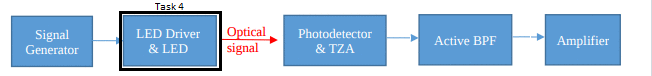
\includegraphics[width=.9\textwidth ]{Introduction/Block_Diagram_MFBP.png}
    \caption{Block diagram for optical uplink \cite{b1}}
    \label{fig:blockdiagram2}
\end{figure}

The output from the the signal generator is not a square wave, nor does it output enough current to drive the LED. The current driver will be created in a subsequent lab. The voltage transfer characteristics (VTC) of an ideal inverter is shown in Figure \ref{fig:vtcideal}.

\begin{figure}[H]
    \centering
    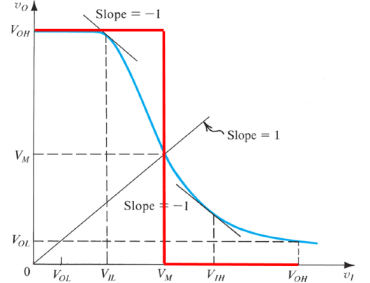
\includegraphics[width=.6\textwidth ]{Introduction/VTC_IDEAL.png}
    \caption{Ideal VTC of inverters \cite{b1}}
    \label{fig:vtcideal}
\end{figure}



\noindent     Figure \ref{fig:vtcideal} describes the ideal VTC of an inverter, where the voltages for logic low and logic high are shown. Both the ring oscillator and the astable multivibrator are created by cascading several CMOS inverters together,

\noindent Section 2 of this report describes the design, and when relevant, the simulations of the NMOS, CMOS inverter, the AND gate, the ring oscillator, and finally the astable multivibrator. Experimental results are addressed in section 3. A discussion of the results, sources of error, and areas of possible improvement are outlined in section 4. Section 5 concludes this report. \newline




\end{document}